\chapter[Introdução]{Introdução}

É inconcebível imaginar o mundo moderno sem software. A sua penetração é tão grande nas mais diversas áreas que seria difícil prever como o mundo seria sem o suporte e as facilidades que ele trás ao nosso dia a dia. Diante desta penetração tão grande e do seu enorme crescimento nos últimos anos, consequência do avanço tecnológico, se torna cada vez mais importante desenvolver software. O desenvolvimento de software pode possuir diferentes contextos de negócio, e com isso diferentes habilidades são exigidas dos desenvolvedores, já que cada contexto possui suas particularidades. Além disso, o ritmo acelerado do mundo moderno faz com que os contextos evoluam, e com isso as suas atividades e necessidades (requisitos) também evoluem. A mudança nos requisitos, a sua diversidade, e em algumas vezes a dificuldade em precisa-los, leva o desenvolvimento tradicional de software a ser lento e caro, em contextos que estão sempre evoluindo \cite{lieberman2006}. Diante deste cenário, se torna cada vez mais comum aplicações de software serem desenvolvidas por desenvolvedores não profissionais, pessoas que possuem expertise em um determinado domínio e que desejam suportar seus objetivos neste domínio através de uma solução computacional \cite{lieberman2006}. O Escritório do Trabalho e Estatística dos Estados Unidos fez uma previsão de que por volta de 2012, nos Estados Unidos, haveriam pouco mais de 3 milhões de programadores profissionais e mais de 55 milhões de pessoas escrevendo fórmulas e \textit{queries} em planilhas e banco de dados, para suportar seus objetivos de trabalho \cite{scaffidi2005}. Um relatório divulgado pelo \textit{Gartner} em Julho de 2011, indicou que desenvolvedores não profissionais iriam construir ao menos 25\% das novas aplicações de negócio em 2014 (Citar fonte - Artigo End User Development, no CEL). Diante deste cenário, um modelo de desenvolvimento de software centrado no usuário final cada vez mais vem ganhando força. O \textit{End User Development} - EUD tem como objetivo oferecer meios para que os usuários finais, que não são especialistas em programação, possam desenvolver aplicações de software. O EUD pode ajudar a aumentar a capacidade produtiva do departamento de TI de uma organização, bem como reduzir custos com o desenvolvimento de aplicações de negócio.

O serviço público brasileiro, por ter natureza administrativa, apresenta grande demanda por desenvolvimento de software. Porém o excesso de burocracia dificulta o aumento da capacidade produtiva da área de TI, que é feita através de concursos ou de contratos terceirizados \cite{artigoTcuGovTI}. Além disso, o uso de planilhas e o desenvolvimento de aplicações clandestinas sem nenhuma documentação e padrão, pelas unidades de negócio, promove o desconhecimento de soluções informatizadas por parte da alta cúpula, bem como a duplicidade de esforços pelas unidades \cite{slideTCU}. Nesse sentido, alguns órgãos da administração pública federal veem reconhecendo esses esforços feitos informalmente pelas áreas de negócio, e começaram a adotar o modelo EUD, com algumas adaptações, para tentar contornar os problemas relatados. Essa adaptação é chamada de modelo de desenvolvimento descentralizado, uma espécie de EUD onde o usuário final não é necessariamente quem desenvolve as aplicações. Geralmente estagiários da área de TI são contratados, para que eles possam ser alocados nas unidades de negócio do órgão, de forma que eles desenvolvam as aplicações junto à área de negócio, com a consultoria técnica da área de TI \cite{slideTCU}. Uma iniciativa bem sucedida de desenvolvimento descentralizado já foi implantada em um órgão da administração pública federal, com um relato de alta satisfação dos usuários. Apesar disso, ainda existem algumas dificuldades no desenvolvimento por parte dos estagiários, que não possuem um guia/processo que os oriente durante todo o ciclo de desenvolvimento. Por serem estagiários, muitos acabam seguindo a forma de desenvolvimento e os padrões que acreditam serem os melhores, o que acaba colocando em dúvida a qualidade de algumas aplicações desenvolvidas. 

\begin{comment}
Apesar disso, existem ainda algumas dificuldades no desenvolvimento por parte dos estagiários desenvolvedores, como a falta de padronização e o que demonstra a necessidade de a elaboração de um processo embasado por princípios em conceitos da engenharia de software, ao mesmo tempo que não seja custoso aos desenvolvedores, já que iria contra a flexibilidade que preconiza o modelo EUD. 
\end{comment}

\citeonline{lieberman2006} relatou que um dos objetivos da interação humano-computador, além de desenvolver sistemas que são fáceis de usar, seria desenvolver sistemas que são fáceis de desenvolver.


\chapter[Referencial Teórico]{Referencial Teórico}

Esta seção apresenta o referencial que embasa este trabalho, de forma a demonstrar o resultado da revisão de literatura feita. O referencial teórico é o meio em que o autor do trabalho demonstra o seu conhecimento sobre uma determinada área de estudo (teorias, vocabulários, variáveis chave, fenômenos, métodos e história) \cite{randolph2009}.

O referencial teórico é composto dos seguintes assuntos: \textit{End User Development}.


\section{\textit{End User Development}}

\textit{End User Development} (Desenvolvimento por usuário final) é um modelo de desenvolvimento de software onde o usuário final é o principal responsável pela construção do software. \citeonline{lieberman2006} define o \textit{End User Development} (EUD) como um conjunto de métodos, técnicas e ferramentas que permitam aos usuários de sistemas de software, que agem como desenvolvedores de software não profissionais, em algum ponto criar, modificar ou estender um artefato de software. Dentre as motivações para este modelo de desenvolvimento, destacam-se a diversidade, a mutabilidade e a dificuldade em precisar requisitos em contextos que evoluam com uma alta frequência, o que pode levar o desenvolvimento tradicional a consumir muito tempo e atingir um alto custo \cite{lieberman2006}. Além disso, uma organização que possui uma demanda por informatização de processos de trabalho, das suas diferentes áreas de negócio, superior a capacidade produtiva da área de TI, pode gerar o não atendimento à certas áreas, por conta das priorizações das demandas \cite{artigoTcuGovTI}. O EUD acelera as respostas às mudanças, porque os usuários finais geralmente são especialistas no domínio em que estão inseridos, e portanto as mudanças nos requisitos são mais facilmente entendidas e absorvidas \cite{fischer2004}. O fato de cada usuário final ser um potencial desenvolvedor também contribui para um aumento da capacidade produtiva da TI.

\begin{comment}
O EUD pode eliminar as potenciais falhas de precisão da informação inerentes ao processo de intercomunicação pessoal, e oferecer respostas mais rápidas à situações onde os requisitos mudam com uma rápida frequência. Isto é possível porque os usuários finais geralmente são especialistas no domínio em que estão inseridos, e portanto as mudanças nos requisitos são mais facilmente entendidas e absorvidas \cite{fischer2004}.
Além disso, as características importantes que motivam esses usuários a se engajarem no desenvolvimento são o empoderamento, a velocidade de desenvolvimento, a flexibilidade e o controle sobre o software \cite{fischer2004}.
\end{comment}



Para que o desenvolvimento seguindo este modelo possa ocorrer é necessário que existam meios para que o usuário final possa desenvolver e adaptar o software, e para tanto a tecnologia envolvida deve diminuir o esforço cognitivo necessário para a construção do software, através da aproximação conceitual entre as ações do mundo real e as do mundo da programação \cite{fischer2004}. Os usuários finais geralmente não possuem habilidades de um profissional da área de software, e também não estão interessados em construir sistemas no mesmo nível que esses profissionais, por isso é necessário que a tecnologia usada no desenvolvimento alinhe a complexidade relacionada a esta atividade com as habilidades do usuário final. Outro ponto importante para fomentar este modelo, é motivar os usuários finais a se engajarem no desenvolvimento, e fatores como o empoderamento, a velocidade de desenvolvimento, a flexibilidade e o controle sobre o software influênciam na motivação desses usuários \cite{fischer2004}. 

O principal objetivo do EUD é oferecer meios para que os usuários finais consigam desenvolver e adaptar software \cite{lieberman2006}. Desta maneira, as aplicações preparadas para o EUD devem ser, principalmente, flexíveis, fáceis de se entender, de se usar, e de se ensinar \cite{lieberman2006}. A preocupação com a tecnologia usada neste modelo de desenvolvimento, mais especificamente na parte das linguagens de programação e aplicações de desenvolvimento, é a relação escopo de aplicação versus esforço de aprendizagem. A figura 1 ilustra a relação do escopo de aplicação e do custo de aprendizagem, para diferentes linguagens de programação e aplicações. Linguagens de programação mais tradicionais como C++ e JAVA oferecem a possibilidade de construção de software de uma grande variedade de domínios, porém a um alto custo associado ao esforço de aprendizagem. Outras linguagens possuem um menor esforço de aprendizagem, ao custo de uma limitação no escopo de aplicação. As linguagens ou aplicações de desenvolvimento ideais para o EUD são as que possuem um alto escopo de aplicação e um baixo esforço de aprendizagem \cite{fischer2004}. As que existem atualmente só utilizam uma pequena parte do potencial do EUD, com algumas falhas \cite{paterno2013}.


\begin{figure}[h]
	\centering
	\label{fig01}
		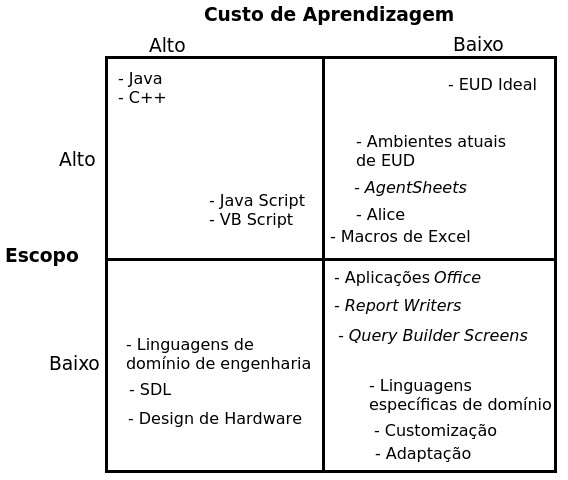
\includegraphics[keepaspectratio=true]{figuras/trade_off_eud_editado}
	\caption{Relação escopo de aplicação e custo de aprendizagem}
\end{figure}
\pagebreak

\citeonline{lieberman2006} classifica as atividades do usuário final em dois tipos:

\begin{enumerate}
\item \textbf{Parametrização ou Customização:} São atividades que permitem o usuário escolher comportamentos, apresentações e mecanismos  alternativos, que já existem dentro de uma aplicação.

\item \textbf{Criação e modificação de programas:} São atividades que implicam na criação ou modificação de artefatos de software. Macros e linguagens de \textit{script} são exemplos deste tipo de atividade.
\end{enumerate}

 
\chapter[Metodologia]{Metodologia}

\citeonline{gil2002} classifica as pesquisas científicas em três grandes grupos, segundo os seus objetivos gerais: exploratórias, descritivas e explicativas.

A pesquisa exploratória tem como objetivo proporcionar o aprimoramento e/ou a descoberta de idéias, a respeito de um determinado problema. Proporcionando uma maior familiaridade com o problema, esse tipo de pesquisa o torna mais explícito e contribui para a construção de hipóteses em cima do mesmo. Por conta disso, a pesquisa exploratória possui um caráter flexível em seu planejamento, e geralmente assume as formas de pesquisa bibliográfica ou estudo de caso \cite{gil2002}.

O estudo de caso consiste no estudo profundo e exaustivo de um ou mais objetos, de forma a obter conhecimento amplo e detalhado sobre o mesmo. Segundo \citeonline{yin2001estudo} o estudo de caso é a abordagem mais adequada para a investigação de um fenômeno em seu contexto real, onde os limites entre este fenômeno e o seu contexto não são claramente percebidos. Os propósitos do estudo de caso são \cite{gil2002}:

\begin{itemize}
\item Explorar situações de contextos reais onde os limites não estão claramente definidos.
\item Preservar o caráter unitário do objeto.
\item Descrever a situação do contexto do qual esta sendo feita a investigação.
\item Desenvolver teorias e formular hipóteses.
\item Determinar as causas de um determinado fenômeno onde a complexidade não permite o uso de levantamentos e experimentos.
\end{itemize}

O conjunto de etapas que podem ser seguidos na maioria das pesquisas classificadas como estudo de caso, bem como uma breve descrição destas etapas são apresentados a seguir \cite{gil2002}.

\begin{enumerate}
\item \textbf{Formulação do problema.}

Constitui a primeira etapa da pesquisa. O problema constitui um fato no qual se deseja aprofundar, de forma a fazer uma descrição de um determinado fenômeno, ou descobrir respostas as causas deste fenômeno. Cuidado deve ser tomado para que o tema seja passível de verificação.

\item Definição da unidade-caso a ser estudada.

A unidade-caso refere-se a um indivíduo num contexto definido. Possui três

\item Determinação do número de casos
\item Elaboração do roteiro.
\item Coleta dos dados.
\item Análise dos dados coletados.
\item Elaboração do relatório.
\end{enumerate}

